%!TeX root=../tese.tex
%(dica para o editor de texto: este arquivo é parte de um documento maior)
% para saber mais: https://tex.stackexchange.com/q/78101/183146

\chapter{Redes neurais no contexto de aprendizado de máquina}
\label{cap:redes}

Neste capítulo são apresentados alguns conceitos básicos de ciência de dados e de aprendizado de máquina, alguns dentre os vários tipos e exemplos de algoritmos de aprendizagem, direcionando-os para aquele que é o foco do trabalho, ou seja, as redes neurais artificiais.



Pode-se classificar as técnicas de aprendizado de várias formas, de acordo com alguma de suas características. Por exemplo, Géron \citep{hands} utiliza o grau de supervisão humana durante o seu funcionamento para classificá-los. Durante o aprendizado podem ou não ser fornecidos um conjunto de consultas e de respostas esperadas. Tais respostas foram dadas por humanos, ao menos neste momento, daí o termo ``supervisão humana''.

Neste texto os termos ``algoritmo'' e ``técnica'' serão usados livremente como sinônimos, pois uma técnica de aprendizado de máquina, no contexto atual, é um algoritmo executado no computador que tem por objetivo ajustar parâmetros de modelos estatísticos.

\section{Tipos de aprendizagem}

 Um algoritmo de \defi{aprendizado supervisionado} é usado quando conhecemos características dos dados que estamos utilizando. De modo geral já temos de antemão as respostas às consultas para os dados utilizados no treinamento. Por exemplo, se estamos classificando fotos de animais, possuímos um conjunto de fotos em que já sabemos quais são de gatos, cachorros, etc.

 O ato de rotular previamente os dados que usamos no treinamento é o que designamos de supervisão humana. Uma vez \emph{treinado}, o algoritmo recebe uma foto, ou seja, uma nova consulta e então fornece a resposta, neste caso se essa é a foto de um gato, ou cachorro, ou qualquer outra resposta dentre aquelas que foram dadas como exemplos durante o treinamento.

Dentro do aprendizado supervisionado temos duas técnicas principais. A primeira é a regressão, usada para prever valores, ou seja, fornecer respostas a consultas ainda inéditas, sejam dados do futuro ou valores de funções em pontos do domínio para os quais ainda não existem respostas. 

A segunda técnica é a classificação, usada para rotular ou dividir os dados em classes pré-determinadas, a partir de exemplos, que é exatamente o caso dos exemplos descritos nos parágrafos anteriores. Se as classes não são conhecidas deve-se utilizar um algoritmo de aprendizado não-supervisionado, descrito na próxima seção.

Enquanto isso, na \defi{aprendizagem não-supervisionada} não sabemos os rótulos dos dados que estamos lidando, assim o algoritmo poderá agrupar os dados de forma automática, por exemplo, se estivermos lidando com problemas de classificação. Aqui, as consultas podem ser coisas como ``quantos são os perfis dos clientes'' ou ``quantas espécies de flores existem nestas fotos'', e assim por diante.

Alguns métodos não-supervisionados de aprendizado foram enumeradas por Géron \citep{hands}. O \textbf{agrupamento} de dados similares sob uma inspiração geométrica. Nesse caso os dados são agrupados conforme suas posições num determinado espaço e utiliza-se algoritmos como $k$-vizinhos, $k$-means, $k$-medians, etc. Exemplos de aplicações são agrupamento de produtos em supermercados, interesses comuns de clientes em sites de conteúdo digital, etc.

Outra técnica é a \textbf{detecção de anomalias}, cujo objetivo é ter uma descrição de como os dados considerados ``normais'' se parecem, e usa-se esse agrupamento para detectar se novos dados estariam ``fora'' desse padrão. Um exemplo é a detecção de fraudes.

Também pode-se citar sobre a técnica de \textbf{estimação de densidades}, que tem como objetivo a estimação da função densidade de probabilidade de um conjunto de dados gerados por algum processo aleatório.

\section{Alguns algoritmos de aprendizagem}

A ideia é descrever nessa ordem:
- aprendizado de maquina
- tipos de aprendizado: supervisionado, não-sup.., semi-sup. e por reforço.
- estratégias com exemplos: vou descrever brevemente, um parágrafo, e exemplificar os que estão aqui \url{https://medium.com/machina-sapiens/algoritmos-de-aprendizagem-de-m%C3%A1quina-qual-deles-escolher-67040ad68737}


\section{As redes neurais e o \emph{perceptron}}

De acordo com Géron \citep{hands}, as primeiras redes artificiais foram introduzidas em 1943 pelo neurofisiologista Warren McCulloch e o matemático Walter Pits através de um modelagem computacional do funcionamento conjunto de neurônios no cérebro de animais, enquanto realizam computações complexas de lógica. Esta foi a primeira \defi{arquitetura} de uma rede neural artificial.

Esse começo promissor levou as pessoas a acreditarem que logo haveriam máquinas realmente inteligentes, o que ficou registrado na cultura da época, principalmente em séries televisivas de ficção científica como \eng{Star Trek} e outras, mas conforme aponta Géron \citep{hands}, essa promessa logo se mostrou inalcansável, ao menos era o que parecia ao final dos anos 60. 

A partir dos anos 80, surgiram novas arquiteturas e melhores técnicas de aprendizagem, embora sua evolução fosse lenta devido ao poder computacional limitado da época. Atualmente, no entanto, isto mudou: há poder computacional em casa e na nuvem, há a internet e fórums de compartilhamento de códigos e conhecimentos em programação e ciência de dados, em resumo o mundo atual está consolidado numa era digital. 

Por essa razão Géron \citep{hands} nos diz que estamos numa nova onda de entusiasmo sobre as redes neurais artificiais, sendo que esse entusiasmo leva o nome de \defi{Deep Learning}, ou aprendizado profundo, e o uso desse adjetivo ajuda a descrever as redes neurais, constituídas de milhares de neurônios, que são utilizadas em várias aplicações de nosso dia-a-dia na internet.

Podemos citar a classificação de bilhões de imagens realizadas pelo \emph{Google}, reconhecimento de fala realizado pela \emph{Siri} da \emph{Apple}, o sistema de recomendações de vídeos do \emph{Youtube} e da \emph{Netflix} e outras plataformas de \emph{streaming}, e até mesmo os jogadores artificiais de xadrex ou do jogo \emph{Go}. As redes neurais artificiais estão vivas em nosso mundo. Mas como funcionam na prática, por detrás dessa aparência de ficção científica?

Uma definição para uma rede neural artificial dada por Rosangela Ballini \citep{doutorado} é a de um sistema de processamento paralelo e distribuído contruído em um formato e com funcionalidade que se parece com o arranjo de um sistema nervoso biológico, sendo compostos por elementos computacionais chamados neurônios, que são organizados e interligados em padrões semelhantes aos neurônios biológicos.

Uma rede neural artificial é um dentre vários métodos de classificação, ou seja, de aprendizado supervisionado, embora ela também possa ser usada para aplicações de aprendizado não supervisionado. De acordo com Kopec \citep{classic}, ele é utilizado como um classificador não-linear, e por isso pode ser utilizado para classificar ou prever quaisquer tipos de funções, que podem ou não ter uma relação linear com o tempo ou com qualquer outro domínio no qual estejam definidas.

Na figura~\ref{fig:neuron} está uma representação de um neurônio biológico. Ele recebe impulsos elétricos de entrada através dos dentritos, que são transmitidos ou não através do núcleo, caso sejam ativados por ele, para os terminais de saída dos axônios. Os neurônios se comunicam através de sinapses, que são ligações entre os dentritos de um e os axônios de outro que realizam a transmissão dos sinais. 

\begin{figure}[htb]
\centering
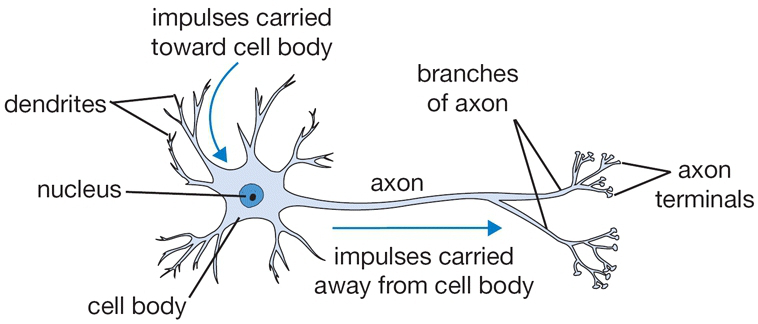
\includegraphics[width=8cm]{figuras/neuron}
\caption{Representação de um neurônio biológico.\footnote{Extraído de \url{https://cs231n.github.io/neural-networks-1/}}}
\label{fig:neuron}
\end{figure}

Dá-se o nome de \eng{perceptron} de camada única (\eng{single-layer perceptron}) ou simplesmente \eng{perceptron} a uma das simples arquiteturas de rede neural artificial, criada em 1957 por Frank Rosenblatt \citep{frank}. Uma ilustração conceitual dela está na figura~\ref{fig:perceptron}. Existem atualmente diversas outras arquiteturas de redes neurais, mas a extensão mais imediata que podemos citar de um perceptron constituído de uma camada de neurônios são as redes \eng{perceptron} multi-camadas (\eng{multi-layer perceptron}). 

Os neurônios são representados por círculos, dentro deles há um valor numérico que intuitivamente podemos atribuir ao nível ou grau de ativação do neurônio, mesmo que no caso biológico se restrinja aos valores $0$ e $1$, ou seja, ativados ou não. Cada coluna de neurônios representa uma camada, nesse caso, da esquerda para a direita temos a camada de entrada, a camada oculta e a camada de saída. As linhas representam as ligações entre os neurônios, sendo que cada neurônio de uma camada está ligado a todos da camada anterior.

\begin{figure}[htb]
\centering
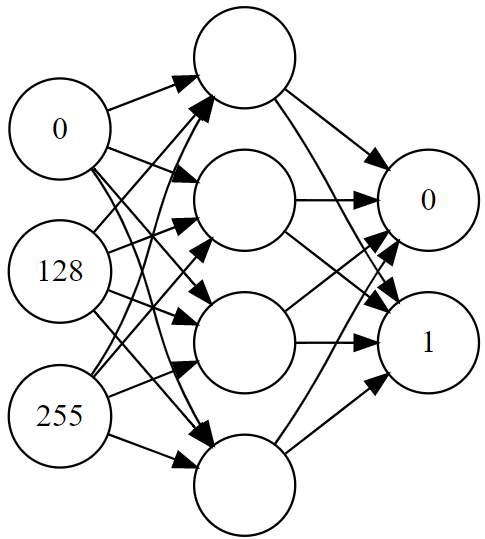
\includegraphics[width=5cm]{figuras/perceptron}
\caption{Rede neural simples, o perceptron de camada única.}
\label{fig:perceptron}
\end{figure}

O perceptron de camada única consiste de uma camada de neurônios de entrada, uma camada oculta de neurônios usados na otimização, e uma camada de saída, que irá conter os dados previstos, ou ainda as probabilidades do dado pertencer a alguma das classes que a rede poderá classificá-lo. E é o fato de haver uma camada oculta nesta rede que a define como sendo de ``camada única''. Caso houvessem mais do que uma camada oculta, ela seria do tipo ``multi-camadas'' mencionada acima.

De modo a entendermos as bases matemáticas do algoritmo, podemos começar de uma rede ainda mais básica, a partir um \eng{perceptron} que seja constituído de apenas $1$ neurônio na única camada oculta. Esta rede super simplificada, que está na figura~\ref{fig:neuronio}, pode ser útil para para o entendimento uma vez que neste caso será possível acompanhar graficamente o resultado da execução do algoritmo.

\begin{figure}[htb]
\centering
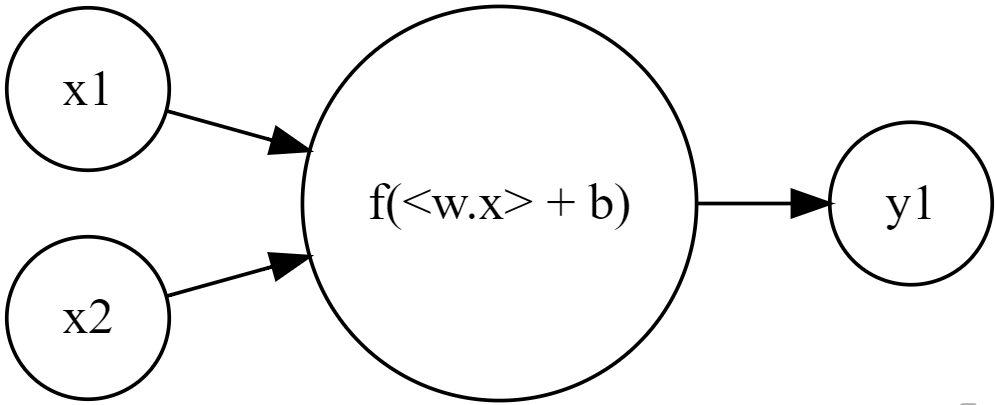
\includegraphics[width=8cm]{figuras/neuronio}
\caption{Rede neural mais simples ainda, apenas um neurônio oculto.}
\label{fig:neuronio}
\end{figure}

Esta rede possui $2$ neurônios na camada de entrada, que são os números reais $x_1$ e $x_2$, $1$ neurônio na camada oculta, no qual está a sua função de ativação $f(x_1w_1 + x_2w_2 + b)$, e $1$ neurônio na camada de saída, que neste caso é um número real $y_1$. Pode-se notar a semelhança dessa rede neural artificial com a sua inspiração biológica com a ajuda da figura~\ref{fig:neuron_model}. 

\begin{figure}[htb]
\centering
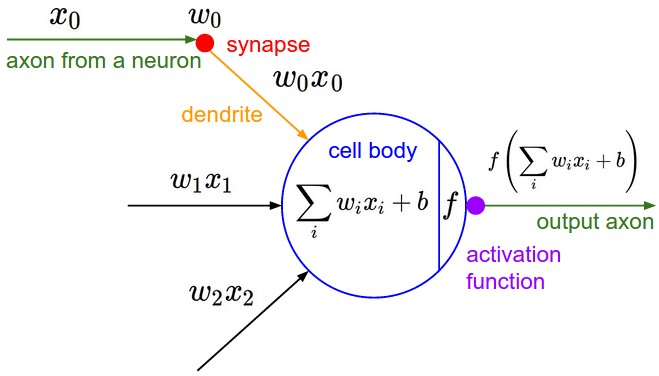
\includegraphics[width=8cm]{figuras/neuron_model}
\caption{Representação de um neurônio artificial.\footnote{Extraído de \url{https://cs231n.github.io/neural-networks-1/}}}
\label{fig:neuron_model}
\end{figure}

Temos os sinais de entrada (como o $x_1$) vindos como viriam os sinais dos axônios de outros neurônios. Eles entram pela camada de entrada da rede, ou dentritos do neurônio. A camada oculta processa as entradas com os pesos, definindo o formato final do sinal através de sua função de ativação, que aqui pode ser uma função real qualquer, mas com funcionalidade similar ao do núcleo do neurônio que ativa/transmite ou não o sinal recebido por ele. Por fim o sinal é enviado à camada de saída, ou aos axônios do neurônio, concluíndo o processamento.

A partir desta analogia podemos compreender o funcionamento básico da rede artificial \eng{perceptron}. Ela recebe uma lista de valores como entrada, que podemos representar por um vetor real $x$. O neurônio oculto representa uma transformação linear neste vetor, que podemos escrever como o produto escalar por um outro vetor real, o vetor de \defi{pesos} $w$, ou seja, $<w.x>$, que é o produto escalar usual dos números reais. A seguir, somamos um outro número real $b$ que é chamado de \defi{viés}, que possui o mesmo papel que a constante de interceptação da reta com o eixo vertical de um ajuste linear.

Por fim, é aplicada uma função de ativação não-linear sobre esta transformação, o que configura a saída deste neurônio: $f({<w.x>} + b)$, que é transmitida ao neurônio de saída, que pode aplicar uma transformação semelhante ou outra qualquer, dependendo da função de ativação utilizada em cada camada da rede. Por simplicidade mostramos uma rede bem simples, mas na prática podem haver muito mais camadas ocultas, e cada uma delas assim como a camada de saída, podem ter muitos neurônios cada.

Este processo de entrada, processamento e saída da rede é chamado de \defi{feedforward}, e consiste no nível mais fundamental do \eng{perceptron}. A partir daí, a forma como a rede será treinada, é o que define se ela será utilizada para um aprendizado supervisionado ou não-supervisionado.

Uma vez que estamos lidando com o aprendizado supervisionado, dever ser utilizado um algoritmo de treinamento que forneça à rede pares conhecidos de vetores de entradas e saídas esperadas, e um \defi{critério de avaliação} de quão boa é a performance da rede para aproximar as suas saídas das saídas esperadas. 

Este critério é uma função que fornece uma medida da distância entre as saídas obtidas pela rede e as saídas esperadas, que é genericamente chamada de função de custo (\eng{cost function}). Se denotarmos por $y$ uma saída conhecida, e por $a^{(L)}$ uma saída obtida pela última camada, exemplos comumente usados são as normas usuais como a distância euclidiana ($(a^{(L)^2} + y^2)^{1/2}$), a função de erro absoluto ($|a^{(L)} - y|$), e a função de erro quadrático médio ($(a^{(L)} - y)^2$) , (\eng{mean square error}, MSE), que é a usada no algoritmo descrito por Kopec \citep{classic} e que será usado neste trabalho.

Um dos algoritmos de treinamento que minimizam uma função de custo é o gradiente descendente (\eng{gradient descent}), que segundo Géron \citep{hands} é um algoritmo muito geral e que serve para encontrar soluções ótimas para uma grande variedade de problemas de otimização. Detalhes de seu funcionamento podem ser vistos no Apêndice \ref{ap:gradiente}.

\section{Outras arquiteturas de redes neurais}

Existem dezenas de arquiteturas de redes neurais artificiais, uma breve olhada na quantidade de arquiteturas listadas no website \emph{The neural network zoo}\footnote{\url{https://www.asimovinstitute.org/neural-network-zoo/}} demonstra que essa brincadeira é levada muito a sério. A representação gráfica ali criada é útil para o entendimento das características das diversas arquiteturas, graças aos padrões de cores e de formas geométricas utilizadas.

A primeira estrutura é o \eng{perceptron} simples, de apenas um neurônio, que processa $n$ entradas através de uma transformação linear seguida de uma função de ativação. É exibido no canto superior esquerdo da Figura \ref{fig:estrutura_p}.

\begin{figure}[htb]
\centering
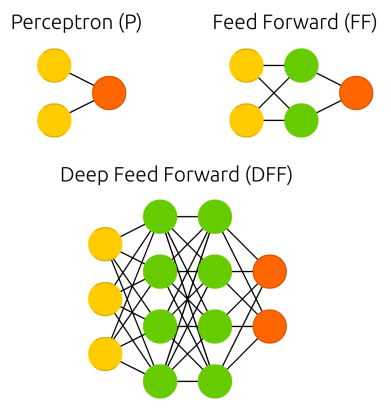
\includegraphics[width=7cm]{figuras/estrutura_p}
\caption{As redes neurais recorrentes: \eng{perceptron}, \eng{feedforward} e \eng{deep feedforward}.\footnote{Extraído de \url{https://www.asimovinstitute.org/neural-network-zoo/}}}
\label{fig:estrutura_p}
\end{figure}

No canto superior direito está a versão \eng{feedforward}, possuindo uma camada oculta(representada pelos círculos verdes), e embaixo está a versão \eng{deep feedforward}, que possui múltiplas camadas ocultas, e número variado de neurônios em todas as camadas, e é de fato a versão que foi implementada nesse trabalho.

As características em comum das arquiteturas derivadas da rede \eng{perceptron}, chamadas de \defi{redes neurais sequenciais}, são a conexão que existe entre cada neurônios de uma camada com todos os neurônios da camada anterior, e a forma que a informação é transmitida da rede, num sentido único, da camada de entrada(os círculos amarelos) para a camada de saída(os círculos vermelhos).

A próxima arquitetura em destaque define o que são as \defi{redes neurais recorrentes}, ilustrada na Figura \ref{fig:estrutura_r}. Nesse tipo de rede a informação pode ir para frente e para trás, além disso pode passar pelo mesmo neurônio oculto mais de uma vez, o que determina o nome recorrente. Esses neurônios são representados pela cor azul na figura.

\begin{figure}[htb]
\centering
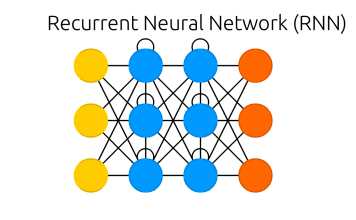
\includegraphics[width=7cm]{figuras/estrutura_r}
\caption{As redes neurais recorrentes.\footnote{Extraído de \url{https://www.asimovinstitute.org/neural-network-zoo/}}}
\label{fig:estrutura_r}
\end{figure}

Esse tipo de rede, segundo Kopec \citep{classic} é o mais usado em problemas em que os dados utilizados possuem uma dependência da ordem em que são obtidos e possuem entradas contínuas, por exemplo, os dados de uma série temporal de dados, ou seja, em que a previsão de um dado , o que representaria o futuro, depende da ordem em que estão os dados já conhecidos, o que representaria os dados do passado.

Outra arquitetura muito utilizada é o das \defi{redes neurais covolucionais}, ilustradas na Figura \ref{fig:estrutura_c}.  Segundo Kopec \citep{classic} essas redes foram projetadas e usadas com sucesso para classificação de imagens ``pesadas'', como fotos de galáxias obtidas em telescópios.

\begin{figure}[htb]
\centering
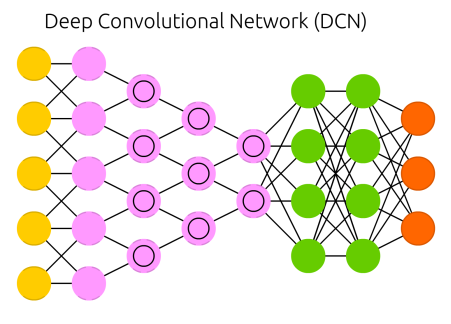
\includegraphics[width=8cm]{figuras/estrutura_c}
\caption{As redes neurais convolucionais.\footnote{Extraído de \url{https://www.asimovinstitute.org/neural-network-zoo/}}}
\label{fig:estrutura_c}
\end{figure}

Em resumo, são redes em que os neurônios de entrada não são conectados totalmente com a primeira camada oculta, mas o que acontece é que vários conjuntos distintos de neurônios da camada de entrada são conectados a várias camadas ocultas separadamente.

A seguir a união dessas camadas ocultas, exibidas como círculos rosas, conectam-se em cascata, perdendo conexões progressivamente até que um número reduzido se conecta a outras camadas, dessa vez camadas ocultas simples, que são os círculos verdes, que conectam-se em formato \eng{feedforward} até o final da rede com a camada de saída. 

Existem ainda outras dezenas de arquiteturas, algumas bem alternativas no formato e nas conexões entre as camadas, fica aqui um único exemplo dentre elas, que é a arquitetura de \defi{redes neurais extremas}. Está ilustrada na Figura \ref{fig:estrutura_e}.

\begin{figure}[htb]
\centering
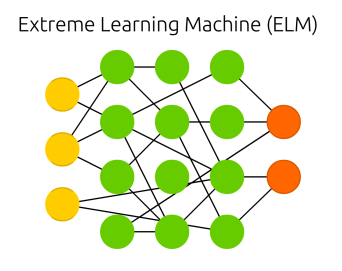
\includegraphics[width=7cm]{figuras/estrutura_e}
\caption{Redes neurais extremas.\footnote{Extraído de \url{https://www.asimovinstitute.org/neural-network-zoo/}}}
\label{fig:estrutura_e}
\end{figure}

As conexões ocorrem de forma não-sequencial, e até mesmo aleatória entre as camadas ocultas, configurando um exemplo curioso de arquitetura, e discussões sobre essas outras arquiteturas não fazem parte do escopo desse trabalho.